\chapter{Search Trees and Fundamentals}\label{ch:foundations}

% [HABICH-R2] KNOWN MATERIAL ONLY: terms, established concepts, existing papers. NO catalogue tables,
% no own conceptual world. Five steps landscape (2.1) -> hardware (2.2) -> workloads/benchmarks (2.3)
% -> software means (2.4) -> notion of heuristics (2.5). All catalogues and own concepts live in Chapter 3.

This chapter leads from the familiar object --- search trees --- via the hardware that shapes their
performance and the workloads under which they are compared, to the software means and the notion of
heuristics by which their design decisions can be abstracted and selected. Everything stays with
\emph{known} terms, concepts, and publications; the systematic catalogues and the thesis's own conceptual
framework follow in Chapter~\ref{ch:measurement}.

\section{Concept and Overview of the State of the Art}\label{sec:overview}
We first map the landscape of search structures --- comparison-based trees, digital and prefix-based methods,
hashing, spatial and flat structures --- and classify the known representatives with their core ideas and
supporting references. The literature refers to the entirety of the best published methods at any given
time as the \emph{state of the art} (SOTA); in this thesis the term always means the published
search-structure designs against which a new design must measure itself. Here it
already becomes apparent that every algorithm can be located in a shared design space; how this design
space is systematically spanned is developed in Chapter~\ref{ch:measurement}.
\begin{figure}[htbp]\centering
\begin{tikzpicture}[font=\footnotesize, align=center, >=Stealth,
  cat/.style={draw, rounded corners, fill=orange!10, inner sep=3pt}]
  \node[cat] (root) at (0,0){search structures};
  \node[cat] (a) at (-5,-1.5){comparison-\\based};
  \node[cat] (b) at (-2.5,-1.5){digital /\\prefix};
  \node[cat] (c) at (0,-1.5){hashing};
  \node[cat] (d) at (2.5,-1.5){spatial};
  \node[cat] (e) at (5,-1.5){flat /\\exotic};
  \foreach \x in {a,b,c,d,e} \draw[->] (root)--(\x);
  \node[font=\scriptsize, text=gray] at (-5,-2.5){B-tree, AVL};
  \node[font=\scriptsize, text=gray] at (-2.5,-2.5){trie, ART, HOT};
  \node[font=\scriptsize, text=gray] at (0,-2.5){Cuckoo, Swiss};
  \node[font=\scriptsize, text=gray] at (2.5,-2.5){R-tree, k-d};
  \node[font=\scriptsize, text=gray] at (5,-2.5){skip list};
\end{tikzpicture}
\caption{The landscape of search structures: five classes with typical representatives.}\label{fig:search-map}
\end{figure}
Search structures can be classified by the mechanism with which they map a key to a
record~\cite{knuth1998taocp3}\@. \emph{Comparison-based} structures locate the key via order comparisons
and presuppose a total order --- from the self-balancing AVL trees~\cite{adelsonvelsky1962avl}, whose
sibling subtrees differ in height by at most one, and the red-black
trees~\cite{bayer1972symmetric,guibas1978redblack}, which secure the same logarithmic height via a node
colouring with looser invariants that are cheaper to maintain, through the block- and
external-memory-oriented
B/B\textsuperscript{+} trees~\cite{bayer1972btree,comer1979btree}, whose nodes typically correspond to a
cache or memory block size~\cite{graefe2001btree,hankins2003nodesize} and which in the
B\textsuperscript{+} variant keep all payload data in the leaves and reduce inner nodes to signposts,
to the main-memory-oriented
T-tree~\cite{lehman1986ttree}, which combines node-local value ranges with AVL balancing and thereby
reduces the number of pointer indirections per search step.\ \emph{Digital} structures, by contrast, branch on the bytes of the key
rather than by comparison, so that the search-path length depends on the key length and not on the
number of keys: the \emph{trie}~\cite{delabriandais1959trie,fredkin1960trie} as the basic form, in which every root
path spells out a key and common prefixes are shared, the
path-compressed radix/PATRICIA trees~\cite{morrison1968patricia} that collapse sparse one-child chains,
and the \emph{Adaptive Radix Tree}
(ART)~\cite{leis2013art}, which adapts the node representation to the actual fanout and serves throughout
this thesis as the reference design.

Beyond the tree-like methods, \emph{hashing} maps keys directly via a hash function and has no inherent
order, which makes range queries expensive~\cite{knuth1998taocp3}; cuckoo hashing~\cite{pagh2004cuckoo},
which unlike open addressing and chaining guarantees constant worst-case lookups, and tables such as
SwissTable~\cite{abseil_swisstable}, which achieve high practical density thanks to SIMD group probing,
stand alongside this work as a
non-tree-like baseline.\ \emph{Spatial} structures (k-d tree~\cite{bentley1975kdtree},
quadtree~\cite{finkel1974quadtree}, R-tree~\cite{guttman1984rtree}) partition a multidimensional key
space and lie outside the scope, as do the theoretical \enquote{exotics} --- the van Emde Boas
tree~\cite{vanemdeboas1975} and the y-fast trie~\cite{willard1983yfast} with $O(\log\log u)$ over a
universe of size~$u$, or the Fusion Tree~\cite{fredman1993fusion} that undercuts the comparison bound ---
as well as the randomized skip list~\cite{pugh1990skiplist}, the flat, sorted array with binary or interpolation search~\cite{knuth1998taocp3} --- strictly speaking the single leaf
of a tree --- and the suffix array, which generalizes this layout on string keys into a space-saving
full-text index and whose lightweight, memory-budgeted construction counts as a textbook example of
algorithm engineering~\cite{manzini2002suffixarray}. This thesis concentrates on the
tree-like structures of the comparison- and digital-based classes (Figure~\ref{fig:search-map}); as
outwardly different as the classes appear, they share recurring, mutually separable partial decisions.

Orthogonal to this search-algorithm view stands the established taxonomy of the \emph{containers} of the
C++ standard library~\cite{iso_cpp}: sequence containers (\texttt{std::vector}) order by insertion
position, ordered-associative ones (\texttt{std::map}, \texttt{std::set}) by key order, unordered ones
(\texttt{std::unordered\_map}) map via a hash function. These standardized interface contracts form the
common basis against which structurally different methods can be measured uniformly --- the ordered map
as the common denominator of a contract shell for comparison- and digital-based search structures, the \texttt{std::vector} as
the sequence view, and the hash table as the unordered counter-check; their placement in the conceptual
framework of this thesis is developed in Chapter~\ref{ch:measurement}.

All methods named so far are \emph{statically designed} structures: their inner organization is fixed
before the first query arrives. An established line of research, by contrast, moves the design into run
time\@. \emph{Database cracking}~\cite{idreos2007cracking} builds the index adaptively as a by-product
of query processing --- each query partitions the data a little further ---, and \emph{stochastic
cracking}~\cite{halim2012stochastic} makes this approach robust against unfavourable query sequences;
\emph{learned indexes}~\cite{kraska2018learned} replace the search structure with a model of the key
distribution that approximately predicts the position of a key. More recent work continues this line in
an actively tuning fashion: VEGA readjusts a learned index at run time with group-wise learning
granularity~\cite{li2025vega}, and AirIndex designs the hierarchy of an index automatically from the
data and storage-I/O profile of the target system~\cite{chockchowwat2023airindex}. These approaches show
a common trend:
away from the hard-wired single structure, towards configurable, self-adapting designs. For the present
thesis they are the closest related known approaches, since they demonstrate that the design decisions
of a search structure can be kept variable; how such decisions can be decomposed systematically and
measured individually is developed in Chapter~\ref{ch:measurement}.

For the cache-related properties of these designs, the literature has developed a graded
terminological taxonomy that this thesis uses throughout. Its starting point is the \emph{I/O model}
(external-memory model) of Aggarwal and Vitter: a two-level memory whose levels exchange data only
in blocks of fixed size; the cost measure of an algorithm is solely the number of block
transfers~\cite{aggarwal1988io}. Transferred to the cache hierarchy, a design is called
\emph{cache-aware} when it knows and explicitly uses the concrete parameters of the target platform
--- block size, capacity; \emph{cache-conscious} has, since Chilimbi, Hill, and Larus, denoted the
same attitude from the data structure's point of view: its layout is deliberately adapted to cache
blocks through clustering, coloring, and compression~\cite{chilimbi1999layout}.
\emph{Cache-oblivious} is the counter-position of Frigo, Leiserson, Prokop, and Ramachandran: the
algorithm knows no parameters at all; analysis takes place in the \emph{ideal-cache model} --- two
levels, capacity~$Z$, line length~$L$, full associativity, optimal replacement ---, and an optimal
cache-oblivious design is then nearly optimal on \emph{every} level of a multi-level hierarchy at
once~\cite{frigo1999cache}.\ \emph{Cache-sensitive}, finally, is the wording of Rao and Ross for
their search trees tailored to the cache line (Section~\ref{sec:hardware-history}) and is used
largely synonymously with cache-aware~\cite{rao1999css,rao2000csb}; as the umbrella term for the
parameter-knowing variants, this thesis uses \emph{cache-aware}.

Orthogonal to this parameter question lies the question of timing: \emph{when} is the cache-related
design decision made? A \emph{static} design fixes it ahead of the first query --- be it
cache-aware on determined parameters or cache-oblivious without parameters ---, whereas the
\emph{active or adaptive} approaches of the previous paragraph move the decision into run time and
readjust it from observed behaviour. Both distinctions --- parameter knowledge and decision timing
--- are independent of each other; the notion of heuristics that later connects them follows in
Section~\ref{sec:heuristics-basics}.

\section{Hardware: Historical Adaptation to Search Performance}\label{sec:hardware-history}
The performance of search structures has always been driven by hardware. We trace the historical advent of
cache-near hardware --- cache hierarchy, cache line, address translation, coherence --- focusing on the
\emph{static and compile-time-relevant} properties that later carry the abstraction in
Section~\ref{sec:software-means}.
\begin{figure}[htbp]\centering
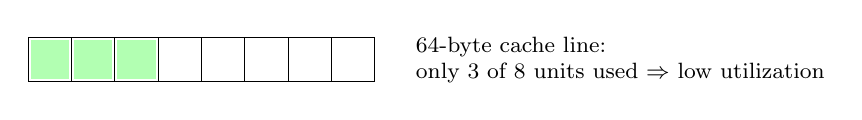
\begin{tikzpicture}[font=\footnotesize, align=center]
  \foreach \i in {0,...,7} { \draw (\i*0.55,0) rectangle (\i*0.55+0.55,0.55); }
  \foreach \i in {0,1,2} { \fill[green!30] (\i*0.55+0.03,0.03) rectangle (\i*0.55+0.52,0.52); }
  \node[anchor=west, align=left] at (4.8,0.27){64-byte cache line:\\only 3 of 8 units used $\Rightarrow$ low utilization};
\end{tikzpicture}
\caption{Cache-line utilization: a cache line is always loaded in full; if only a few of its bytes are used, effective bandwidth drops --- cache-aware layout raises utilization.}\label{fig:cache-line}
\end{figure}
Modern processors interpose several cache levels (L1, L2, and --- not on every platform --- L3) between
the registers and main memory~\cite{hennessy2019architecture}; an access that finds its datum nearby is
cheap, whereas a miss down to main memory costs several hundred cycles~\cite{drepper2007memory}, on
multi-socket and chiplet systems additionally depending on the owning NUMA node. The transfer unit between the levels
is the \emph{cache line} (Figure~\ref{fig:cache-line}); its size is no universal constant but hard-wired
per microarchitecture --- 64\,bytes on x86-64 and common ARM cores (such as Cortex-A76 or Neoverse~V2),
128\,bytes on Apple Silicon L2 and system-level cache~\cite{apple_optimization},
narrower 32\,bytes on older or embedded
cores~\cite{hennessy2019architecture,intel_optimization,amd_sog}. Programs can
\emph{read} it at runtime --- via \texttt{CPUID} (x86), \texttt{CTR\_EL0} (ARM), or \texttt{riscv\_hwprobe}
(RISC-V\@; restricted, among other things to CBO block sizes)~\cite{arm_arm,intel_sdm} --- but not change
it; the depth of the hierarchy also varies (simple
RISC-V cores such as the SiFive~U74 end at L2, some AMD processors bring a stacked 3D V-Cache L3). For a
cache-line-aware layout,
the line size determined per target platform is therefore an \emph{input to compilation}, not a fixed
assumption. Moreover, the transfer of a line does not proceed strictly block-at-once: \emph{critical-word-first} delivers
the requested word first, and DDR5 splits the memory channel into two independent 32-bit
sub-channels~\cite{micron_ddr5}; non-temporal or write-combining stores additionally bypass the normal
write-allocate path instead of pulling the affected cache line into the cache
hierarchy~\cite{intel_sdm}.

\subsection{Cache Organization: Associativity, Miss Classes, and Parallelism}\label{subsec:cache-organisation}
Where a line may reside in the cache is determined by \emph{associativity}: the cache is organized
into \emph{sets}, each holding $n$ \emph{ways} (line slots); the memory address decomposes into tag,
set index, and line offset, and each address may reside only in the $n$ slots of \emph{its} set ---
direct-mapped ($n=1$) and fully associative (a single set) are the limiting cases, and common data
caches lie in between at 4- to
16-way~\cite{hennessy2019architecture,intel_optimization,amd_sog}. By their cause, Hill and Smith
classify misses into three classes (the \emph{3-C model}): \emph{compulsory} (first access --- the
line was never in the cache), \emph{capacity} (the working set exceeds the capacity), and
\emph{conflict} (more hot lines fall onto one set than it has ways)~\cite{hill1989associativity};
the textbook presentation adds \emph{coherence} misses as a fourth class in multi-core
systems~\cite{hennessy2019architecture}. The classification is more than bookkeeping, since it
separates the countermeasures: compulsory misses are addressed by prefetching
(Section~\ref{subsec:prefetching}), capacity misses by more compact layouts, and conflict misses
arise precisely with the regular address patterns of large node arrays --- if hot elements lie
apart at power-of-two distances, they compete for the same
sets~\cite{hennessy2019architecture,drepper2007memory}.

Moreover, a miss does not block a modern cache: since Kroft's \emph{lockup-free} organization, the
cache keeps one status register per outstanding miss (\emph{miss status holding register}, MSHR)
and serves further accesses in the meantime~\cite{kroft1981lockupfree}. The small, fixed number of
these registers --- realized at Intel as \emph{line fill buffers} between L1 and L2 --- limits how
many memory accesses can be in flight at once: the \emph{memory-level parallelism}
(MLP)~\cite{hennessy2019architecture,intel_optimization}. Whether a search structure can offer this
parallelism at all is a design question --- the search path of a tree is a chain of mutually
dependent accesses and does not exploit it as a matter of course
(Section~\ref{subsec:prefetching}).

Two further properties act at the line boundaries: \emph{alignment} --- an object spanning a line
boundary costs two transfers instead of one, which is why cache-aware layouts align nodes to line
boundaries --- and \emph{false sharing}: if two cores write to \emph{disjoint} fields of the same
line, the line migrates back and forth between the cores despite logical independence, because
coherence (Section~\ref{subsec:write-coherence}) always manages whole
lines~\cite{drepper2007memory,intel_optimization}.

\subsection{Cache-Line-Oriented Layout Research}\label{subsec:layout-research}
This very cache-line-oriented layout is the historical guiding idea of the relevant research: the CSS
tree~\cite{rao1999css} introduces the cache-line node, the CSB\textsuperscript{+} tree~\cite{rao2000csb}
the contiguous sibling cluster, Hankins and Patel~\cite{hankins2003nodesize} measure the effect of node
size, and Samuel et al.~\cite{samuel2005procaware} make the node processor-aware; the Adaptive Radix
Tree~\cite{leis2013art} grades node size cache-line-orientedly with Node4/16/48/256, and Schmidt et
al.~\cite{schmidt2025hbm} measure stride versus sequential accesses on high-bandwidth memory. As
concrete layout options, the literature knows the dense and the cache-line-aligned array-of-structs,
the column-oriented struct-of-arrays, the bit-packed LOUDS~\cite{jacobson1989louds}, and the SIMD-tiled
AoSoA. The multi-level hierarchy itself is moreover the subject of software/hardware-cooperative
prefetching methods such as the hierarchical instruction prefetcher for server applications of Zhang et
al.~\cite{zhang2025hierarchical}, which enters this thesis as a prefetching instance and not as a data-structure-specific
tree data prefetch.

\subsection{Prefetching}\label{subsec:prefetching}
Prefetching brings data into the cache \emph{before} their use and is the primary countermeasure
against compulsory misses and unhidden memory latency
(Section~\ref{subsec:cache-organisation}). The hardware prefetchers of modern cores form a few
documented classes: next-/adjacent-line prefetchers fetch the neighbouring line of every missed
line, stream prefetchers detect ascending or descending access sequences and run ahead of them,
stride prefetchers learn constant distances per load instruction (recognized by instruction
pointer), and more complex spatially or temporally correlating methods are the subject of research;
the survey is given by Mittal~\cite{mittal2016prefetching}, and the concrete prefetchers of the
L1/L2 stages are documented in the vendor manuals~\cite{intel_optimization,amd_sog}. A prefetcher
is judged by three quantities: \emph{accuracy} (how many fetched lines were used), \emph{coverage}
(how many misses were avoided), and \emph{timeliness} --- prefetches that come too late hide the
latency only partially, those that come too early evict lines still
needed~\cite{mittal2016prefetching}.

In addition, the architectures provide \emph{software} prefetch instructions (x86: the
\texttt{PREFETCHh} family including a non-temporal variant; ARM\@: \texttt{PRFM}) with which the
program itself announces an address together with a target level~\cite{intel_sdm,arm_arm}. Their
central tuning knob is the \emph{prefetch distance} --- how far ahead the announcement is made:
large enough to hide the memory latency, small enough not to lose the fetched line again before
use; it depends on latency and processing speed and is thus a quantity to be calibrated per
platform~\cite{mittal2016prefetching}. In index research, Chen et al.\ justify wider
B\textsuperscript{+} nodes precisely for this reason: if all lines of a multi-line node are announced
in parallel, the effective node load time drops, and the optimal node width grows beyond the single
cache line~\cite{chen2001prefetch}; fractal prefetching transfers the same principle across levels
to disk pages~\cite{chen2002fractal}.

Prefetching finds its limit at \emph{pointer chasing}, the core of every tree search: the address
of the next node is known only once the line of the current node has arrived. Such a dependent load
chain offers no pattern to either a stride or a stream prefetcher, and it serializes the memory
accesses --- the available memory-level parallelism (Section~\ref{subsec:cache-organisation})
remains unused~\cite{mittal2016prefetching}. The known countermeasures therefore start not at
prediction but at design: more useful bytes per dependent step (wider, line-aligned
nodes~\cite{chen2001prefetch}) or several \emph{independent} searches whose accesses are
interleaved so that the load chain of one fills the waiting time of the others --- design answers
that recur as parameters in Section~\ref{subsec:cc-structures}.

\subsection{Main Memory and Address Translation: DRAM, NUMA, and TLB}\label{subsec:memory-numa-tlb}
Behind the last cache lies the DRAM main memory, whose characteristics the JEDEC standard fixes for
the current generation DDR5 (JESD79-5)~\cite{jedec_jesd79_5}. Two quantities are frequently
conflated: the \emph{data rate} in megatransfers per second (MT/s\@; two transfers per clock)
measures the bandwidth of the interface, while the \emph{CAS latency} (CL) counts clock cycles
until the first response of an opened row --- since the CL cycle count grows with the nominal rate,
rising data rates hardly lower the absolute access
latency~\cite{hennessy2019architecture,micron_ddr5}. Parallelism is supplied by the organization:
several memory channels per system, the already-mentioned DDR5 split of each channel into
independent 32-bit sub-channels, and bank groups within each chip whose interleaved operation
covers row activation times~\cite{jedec_jesd79_5,micron_ddr5}. Stored on the module are the
standard's \emph{JEDEC nominal profiles}; alongside them exist vendor-specific overclocking
profiles (Intel XMP, AMD EXPO) beyond the standard rates --- which rate a machine actually runs is
therefore a property of the target platform that must be documented, not a constant readable from
the module.

In multi-socket and chiplet systems, topology is added: with \emph{NUMA} (non-uniform memory
access), each node owns local memory, and accesses to remote nodes cost noticeably more than local
ones. By default the operating system places pages according to the \emph{first-touch} policy ---
a page ends up on the node of the thread that first writes it~\cite{lameter2013numa}. For
measurements on search structures this is a silent precondition: whoever builds the structure on a
different node than the one measuring it measures the interconnect latency as well.

Besides the data-cache hierarchy there exists a second locality boundary: the \emph{translation lookaside
buffer} (TLB) caches virtual-to-physical mappings, and a TLB miss triggers an expensive page
walk~\cite{hennessy2019architecture}. Its \emph{reach} --- entry count times page size --- limits
the memory region addressable without a page walk. For locality reasons processors separate the instruction TLB from
the data TLB (dTLB) --- since instruction accesses are considerably more local than data accesses ---
and lay it out in multiple stages (L1 dTLB plus a shared L2 STLB)~\cite{intel_sdm,drepper2007memory}; for search
structures the dTLB is the second, independent boundary alongside the cache line, since large or widely
scattered nodes raise dTLB pressure independently of cache utilization. In the state of the art the dTLB appears mainly as a
\emph{measurement target}; algorithmically it is addressed by large pages (huge pages, 2\,MiB/1\,GiB),
which enlarge the TLB reach, are supported by several allocators
(mimalloc, jemalloc, TCMalloc, snmalloc), and which Schmidt et al.~\cite{schmidt2025hbm} use
empirically with 2-MiB pages --- a standalone dTLB optimization nevertheless remains
underrepresented in the search-algorithm papers, an observation to which the research gap in
Chapter~\ref{ch:measurement} (Section~\ref{sec:task-concerns}) returns.

\subsection{Write Path, Replacement, and Coherence}\label{subsec:write-coherence}
The write and update behaviour of the caches, too, is largely microarchitecturally fixed. Writes follow
\emph{write-through}, which writes immediately through to the next level, or \emph{write-back}, which at
first merely marks the change in the cache line (\emph{dirty}) and writes it back only upon its eviction
--- which saves bus traffic and lowers write latency; orthogonally to this the allocation policy
(write-allocate, typical with write-back, or
no-write-allocate, typical with write-through) determines the handling of a write miss; ARMv8 makes this
choice explicit via page
attributes --- write-through, write-back, or non-cacheable together with read- or read-write-allocate
hints ---~\cite{arm_arm}, while x86 normally uses write-back with write-allocate~\cite{intel_sdm}. Which
line is evicted is decided by a heuristic replacement strategy from LRU/pseudo-LRU to the two-bit-frugal,
scan- and thrash-resistant
\emph{re-reference interval prediction} (dynamic variant DRRIP)~\cite{jaleel2010rrip}, which builds on
the adaptive insertion policy~\cite{qureshi2007adaptive}; how many levels hold a
line at once is governed by the inclusion policy --- an \emph{inclusive} cache holds every line of the
higher levels redundantly, an \emph{exclusive} one (victim cache) excludes them, a \emph{non-inclusive}
one allows both ---, and in multi-core systems an invalidation-based
coherence protocol secures consistency: the widespread MESI keeps every line in one of the states
\emph{Modified}, \emph{Exclusive}, \emph{Shared}, or \emph{Invalid}, extended by vendors with variants
such as MOESI (AMD~\cite{amd_sog}) or MESIF
(Intel~\cite{intel_optimization})~\cite{hennessy2019architecture}. As a concrete instance of these fixed
properties, the L3
inclusion policy varies between generations --- inclusive on earlier Intel client generations (such as
Nehalem), non-inclusive on
Intel servers from Skylake-SP/Xeon~Scalable, and predominantly victim-like on
AMD~Zen~\cite{intel_optimization,amd_sog}.
Since for the most part this is not freely selectable at runtime, these properties are given per target platform and
accessible only through measurement; their effect --- in particular the \emph{cache-line ping-pong} under
competing writes to the same line --- must be made visible explicitly by a fair measurement procedure
(Chapter~\ref{ch:measurement}).

\subsection{Cache-Aware and Cache-Oblivious Data Structures}\label{subsec:cc-structures}
With the terminological taxonomy from Section~\ref{sec:overview} and the parameters now introduced,
the state of the art of cache-near data structures can be ordered. The empirical impulse of the
cache-aware line was given by Ailamaki et al., whose time breakdown of commercial database systems
showed that around half of the execution time lies in memory stall cycles --- above all in L2 data
and L1 instruction misses~\cite{ailamaki1999dbms}. The answers of the following years each bind
part of the parameters from the previous sections explicitly into the design: the cache-line size
(CSS/CSB\textsuperscript{+} tree~\cite{rao1999css,rao2000csb}), the prefetch distance together with
multi-line nodes (pB\textsuperscript{+} tree~\cite{chen2001prefetch}, across levels fractal
prefetching~\cite{chen2002fractal}), page size and SIMD width at once (FAST, an
architecture-sensitive tree layout with interlocked page, line, and SIMD
blocking~\cite{kim2010fast}), or the fanout per cache line (ART~\cite{leis2013art}); the layout
techniques of clustering and compression go back to Chilimbi et al.~\cite{chilimbi1999layout}. The
cache-oblivious counter-position is instantiated as well: Bender et al.\ ground the cache-oblivious
B-tree on the van Emde Boas layout~\cite{bender2005coboblivious}, building on the
order-maintenance/packed-memory primitive~\cite{bender2002orderlist}, the cache-oblivious traversal
of ordered sets with a locality-preserving $O(k/B)$ bound~\cite{bender2002scanning}, and the layout
of a tree of fixed topology that minimizes the expected number of block transfers in a multi-level
memory model nearly optimally even under unknown block
size~\cite{bender2002treelayout,bender2000cobtree}; Saikkonen and Soisalon-Soininen maintain a
cache-sensitive layout invariant even under
updates~\cite{saikkonen2008multilevel,saikkonen2016layout}, and
Graefe/Larson~\cite{graefe2001btree} compare both approaches across the CPU cache levels, while all
practical trie and B\textsuperscript{+} indexes are designed cache-aware.
Table~\ref{tab:structure-parameters} orders the designs named here by which hardware parameters
they explicitly bind into the design.

\begin{table}[!htbp]
  \caption{Cache-near structure designs and the hardware parameters they explicitly bind into the
  design.}\label{tab:structure-parameters}
  \centering\footnotesize
  \begin{tabular}{@{}l c c c c c@{}}
    \toprule
    \textbf{Design} & \textbf{Cache line} & \textbf{Page/TLB} & \textbf{SIMD width} &
    \textbf{Prefetch distance} & \textbf{parameter-free} \\
    \midrule
    CSS tree~\cite{rao1999css}                         & $\bullet$ & ---       & ---       & ---       & --- \\
    CSB\textsuperscript{+} tree~\cite{rao2000csb}      & $\bullet$ & ---       & ---       & ---       & --- \\
    pB\textsuperscript{+} tree~\cite{chen2001prefetch} & $\bullet$ & ---       & ---       & $\bullet$ & --- \\
    Fractal prefetching~\cite{chen2002fractal}         & $\bullet$ & $\bullet$ & ---       & $\bullet$ & --- \\
    FAST~\cite{kim2010fast}                            & $\bullet$ & $\bullet$ & $\bullet$ & ---       & --- \\
    ART~\cite{leis2013art}                             & $\circ$   & ---       & $\bullet$ & ---       & --- \\
    Cache-oblivious B-tree~\cite{bender2005coboblivious} & ---     & ---       & ---       & ---       & $\bullet$ \\
    Node-size study Hankins/Patel~\cite{hankins2003nodesize} & $\bullet$ & --- & ---       & ---       & --- \\
    \bottomrule
  \end{tabular}
  \par\medskip\footnotesize
  Legend: $\bullet$ = explicit design parameter of the original work; $\circ$ = considered
  indirectly (ART grades its node sizes cache-line-orientedly without parameterizing the line
  size); --- = not addressed. Classification by this thesis based on the cited original works.
\end{table}

Two observations on the table carry further. First, every design binds a \emph{handful} of
parameters firmly --- no known design treats the parameter set of the previous sections as an open
input space. Second, both philosophies leave the same question open: how can \emph{measured}
locality knowledge of the concrete target platform --- whose cache properties are predominantly
hard-wired and only to a lesser extent configurable (Section~\ref{subsec:write-coherence}) --- be
combined systematically with the cache-near settings that are actually selectable? This question is
taken up again in Chapter~\ref{ch:measurement} (Section~\ref{sec:task-concerns}).

\section{Workloads and Benchmark Conventions}\label{sec:workload-basics-known}
Whether a search structure makes good use of the hardware properties from
Section~\ref{sec:hardware-history} only shows under load; for this, fixed terms and benchmark
conventions have become established. A \emph{load} (operation) is a single call of the search
interface --- a point query, an insertion, a deletion, or a range scan. A \emph{workload} (in this
thesis synonymously: \emph{load profile}) is a
structured profile of such operations: an operation mix (e.g.\ 50\,\% read / 50\,\% update) over a key
access distribution (uniform, Zipf-distributed, latest values) on a dataset of defined size and key
characteristic. Realistic workloads are thereby sequences of many consecutive interface calls
--- not isolated, unrealistic single accesses.

The most widespread workload convention is the Yahoo!\ Cloud Serving Benchmark
(YCSB)~\cite{cooper2010ycsb}. It defines a family of key-value workloads: YCSB-A (50/50 read/update,
Zipf-distributed), YCSB-B (95/5 read/update), YCSB-C (read only), YCSB-D (latest values), YCSB-E
(short range scans), and YCSB-F (read-modify-write). Alongside this, the literature relies on further
established families: the index benchmark \emph{SOSD}~\cite{kipf2019sosd}, the benchmarks
of the \emph{TPC} family (transactional TPC-C, analytical TPC-DS)~\cite{tpc_benchmarks}, the integration into real systems (such
as SuRF~\cite{zhang2018surf} as a Bloom-filter replacement in RocksDB), real string corpora (URLs, DNA,
dictionary terms), and --- for the hardware-near works --- \emph{SPEC~CPU}~\cite{spec_cpu2017} and
\emph{CloudSuite}~\cite{ferdman2012cloudsuite}. These frameworks produce different loads that are not
directly comparable with one another.

The \emph{goal of workload variation} is to break a methodological bias: each publication typically
chooses the load profile under which its own algorithm performs best. Only when all load profiles run
against all comparison candidates can bias-reduced comparability be gained. For this thesis, the
conventions named above provide the raw material of a common set of load profiles; how this set is
constructed and driven over all candidates is developed in Chapter~\ref{ch:measurement}, and the
corresponding measurement matrix belongs to the evaluation methodology (Chapter~\ref{ch:eval}).

Observation under load uses an established set of metrics. At the cache level one counts the misses
per level, expressed as a \emph{miss rate} (misses per access) or --- more robust when comparing
programs of different access intensity --- as \emph{MPKI} (misses per thousand instructions); at
the core level, \emph{IPC} and \emph{CPI} (instructions per cycle and its reciprocal) measure the
achieved execution density, and stall-cycle breakdowns show which share of the clock cycles is
spent on waiting memory accesses~\cite{hennessy2019architecture}; that this share can dominate
under database loads was precisely the finding of Ailamaki et al.~\cite{ailamaki1999dbms}
(Section~\ref{subsec:cc-structures}). For cache-aware layouts, the \emph{cache-line utilization} is
added --- the share of actually used bytes per loaded line (Figure~\ref{fig:cache-line}) --- which
directly measures what a layout gains at the transfer unit.

These quantities are collected via the processors' \emph{performance monitoring counters} (PMC): a
few programmable count registers per core to which a hardware event (such as an L2 miss or a dTLB
miss) is assigned via event selection; they are made accessible by tools such as
\texttt{perf}~\cite{demelo2010perf} or VTune~\cite{reinders2005vtune}. Their limits are just as
well documented: counter values are not strictly deterministic across repetitions and, depending on
the event, systematically overcount~\cite{weaver2008counters}, and if more events are to be
observed than registers exist, the tool multiplexes the counters --- the result is then an
extrapolation, not a count. A reliable comparison therefore needs repetitions and an honest
statement of dispersion~\cite{hoefler2015benchmarking,weaver2008counters}. Which of these metrics
this thesis collects and how they are ordered into measurement categories is developed in
Chapter~\ref{ch:measurement}.

\section{Software Means and Synthesis into the Abstraction}\label{sec:software-means}
With which software-system means --- compile-time metaprogramming, static use of the hardware
properties from Section~\ref{sec:hardware-history} --- can the abstraction left open there be
\emph{realized}? Available are the
established means of software-engineering design: the named design
patterns~\cite{gamma1994patterns}, the static polymorphism of the \emph{Curiously Recurring Template
Pattern} together with \emph{policy-based design}~\cite{alexandrescu2001modern}, and the composition from
interchangeable building blocks as described by invasive software composition from gray-box
components~\cite{assmann2003invasive}, generative programming~\cite{czarnecki2000generative}, and the
feature-oriented software product lines~\cite{apel2013feature,batory1992hierarchical}; C++23 modules
structure the translation units of such building-block compositions but by themselves do not yet guarantee portable ABI
stability~\cite{wg21_modules_abi} --- relevant as soon as pre-compiled building blocks are to be
exchanged.

For interchangeable building blocks to become a concrete system, what is needed besides the
composition techniques is a \emph{form of description} for the configuration chosen in each case.
The established answer are \emph{declarative configuration models}: feature models have described
configurable variant spaces as feature hierarchies with selection constraints since the FODA
study~\cite{kang1990foda}, generative programming produces the system variant in the solution
space from such configuration knowledge in the problem space~\cite{czarnecki2000generative}, and
the product-line literature systematizes the associated binding times from compile time to run
time~\cite{apel2013feature}. Industrial tooling follows the same principle: Maven's \emph{Project
Object Model} is the declarative --- held as an XML file --- manifestation of \emph{what} makes up
a modular Java system, while the build lifecycle takes over the \emph{when} and
\emph{how}~\cite{maven_pom}; CMake produces a native buildsystem per platform from one declarative
description via interchangeable \emph{generators}~\cite{cmake_manual}; and Mokhov, Mitchell, and
Peyton Jones show that build systems as a whole can be scientifically captured and recombined as a
combination of a few scheduler and rebuilder building blocks over declarative dependency
descriptions~\cite{mokhov2018build}. That declarative models can accompany a system beyond build
time into operation is developed by the models@run.time line~\cite{blair2009modelsruntime}; Götz
shows in the TU Dresden MQuAT dissertation how declarative (configuration) models steer the
self-optimization of component-based systems through contract negotiation~\cite{goetz2013mqat}.

For this thesis, both strands together form the toolbox: the composition techniques with which the
hardware properties measured per target platform can be turned into a concrete layout at compile
time, and the declarative configuration models with which the chosen configuration can be described
and reproduced; how both are combined for this purpose is developed in
Chapter~\ref{ch:measurement}.

\section{Heuristics as Decision Rules}\label{sec:heuristics-basics}
Both the adaptive and learned indexes (Section~\ref{sec:overview}) and the replacement strategies of
the caches (Section~\ref{sec:hardware-history}) make their decisions \emph{heuristically}. A
\emph{heuristic} is a decision rule without a guarantee of optimality: it maps observable features ---
such as the cache properties determined per target platform (Section~\ref{sec:hardware-history}) or
the measured load profile (Section~\ref{sec:workload-basics-known}) --- to a concrete configuration
without proving that configuration best. It takes the place of an exact solution wherever the latter
is unknown or too expensive to determine; the cache's own heuristic replacement strategies (LRU,
RRIP\@; Section~\ref{sec:hardware-history}) are the hardware-side archetype of this way of
thinking~\cite{jaleel2010rrip}.

Heuristics can be distinguished by \emph{when} their decision is made. A \emph{static heuristic} is
fixed at compile time: the chosen configuration is compiled firmly into the translated program and no
longer changes at run time. A \emph{dynamic heuristic}, by contrast, selects the configuration at run
time, depending on the actually observed behaviour, and may adjust it during operation. Both variants
presuppose the same \emph{heuristic function} but shift the moment of its evaluation.

Formally, this heuristic function is a \emph{mapping} from a measurement result or load profile to a
configuration: $h: \mathcal{M} \rightarrow \mathcal{K}$, where $\mathcal{M}$ denotes the space of
collected features (measurements, load-profile metrics) and $\mathcal{K}$ the space of admissible
configurations. The present thesis first measures this relationship systematically
(Chapter~\ref{ch:measurement}); the \emph{automated} determination of $h$ itself --- the mechanism
that derives the respective best configuration from the measurement results --- is an objective and
outlook of this thesis (Section~\ref{sec:outlook}).

Finally, the terms used partly synonymously in the literature must be delimited\@. A heuristic is
called \emph{adaptive} if it adjusts its decision to changing conditions; \emph{dynamic} refers more
narrowly to the moment --- evaluation at run time rather than at compile time; and
\emph{measurement-driven} emphasizes the data source --- the decision rests on collected measurements
rather than on fixed model assumptions. An adaptive heuristic is thus always dynamic, a dynamic one
not necessarily adaptive, and both may, but need not, be measurement-driven.

With this, the foundations are assembled: the landscape of search structures, the hardware properties
that shape their performance, the workload conventions under which they are compared, the software
means of abstraction, and the notion of heuristics that connects measured knowledge with configuration
choice. How exactly these means allow a search algorithm to be decomposed into orthogonal, individually
measurable design decisions is developed in Chapter~\ref{ch:measurement}; the concrete realization of
the building blocks introduced there is shown in Chapter~\ref{ch:impl}.
